\subsection{Charakterisierung des Pr:YLF-Kristalls}

\subsubsection{Absorptionsspektrum}

Zur Bestimmung des Absorptionsspektrums des Pr:YLF-Kristalls wurde mit dem USB-Spektrometer ein
Referenzspektrum aufgezeichnet (Tageslicht vom Himmel), dann das Transmissionsspektrum des Kristalls
mit dem gleichen Licht aufgezeichnet und (vom Spektrometer) das Absorptionsspektrum als Differenz
berechnet.
Abb.~\ref{img:AbsSpec} zeigt das berechnete Spektrum.
Die Lage der Absorptionsmaxima ist eingezeichnet und in Tab.~ \ref{tab:AbsSpec} aufgeführt.

\begin{figure}[H]
\begin{center}
  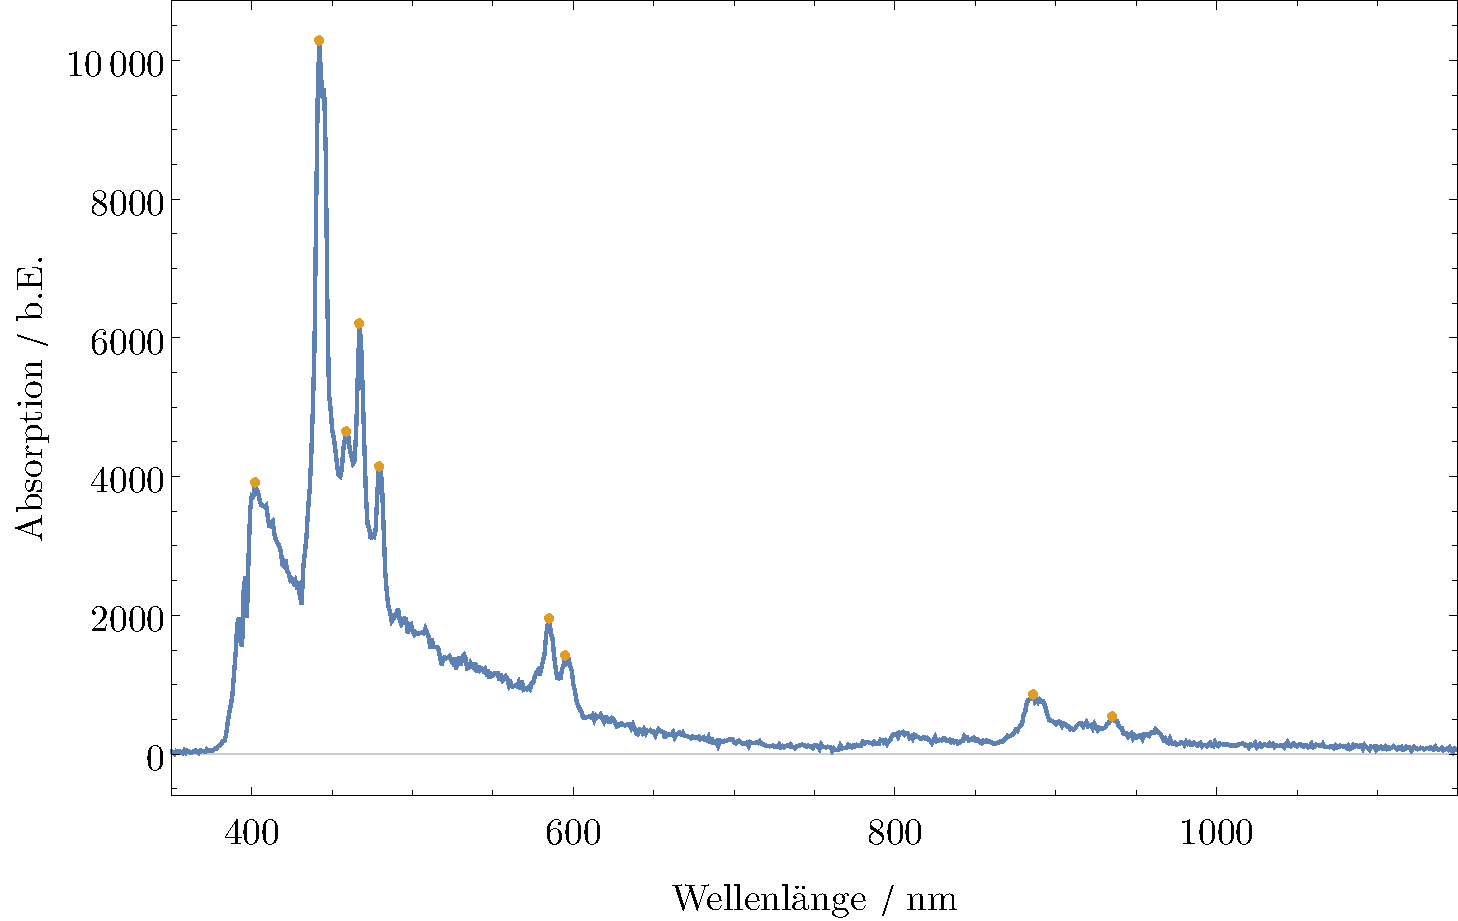
\includegraphics[width=\textwidth]{AbsSpec.pdf}
  \caption{Absorptionsspektrum des Pr:YLF-Kristalls und Position der Maxima.}
  \label{img:AbsSpec}
\end{center}
\end{figure}

\begin{table}[htb]
\caption{Positionen und relative Intensitäten der Absorptionsmaxima im Spektrum des
Pr:YLF-Kristalls.}
\begin{center}
\begin{tabular}{|c|c|}
\hline
Wellenlänge / nm & Absorption / b.E. \\ \hline
402 & 3918.9 \\ \hline
442 & 10287.3 \\ \hline
459 & 4653.3 \\ \hline
467 & 6203.5 \\ \hline
479 & 4147.4 \\ \hline
585 & 1947.5 \\ \hline
595 & 1420.8 \\ \hline
886 & 850.9 \\ \hline
935 & 535.6 \\ \hline
\end{tabular}
\end{center}
\label{tab:AbsSpec}
\end{table}


\subsubsection{Emissionsspektrum}

\paragraph{Aufbau und Durchführung}
blablabla

\paragraph{Auswertung}

blablabla

\begin{figure}[H]
\begin{center}
  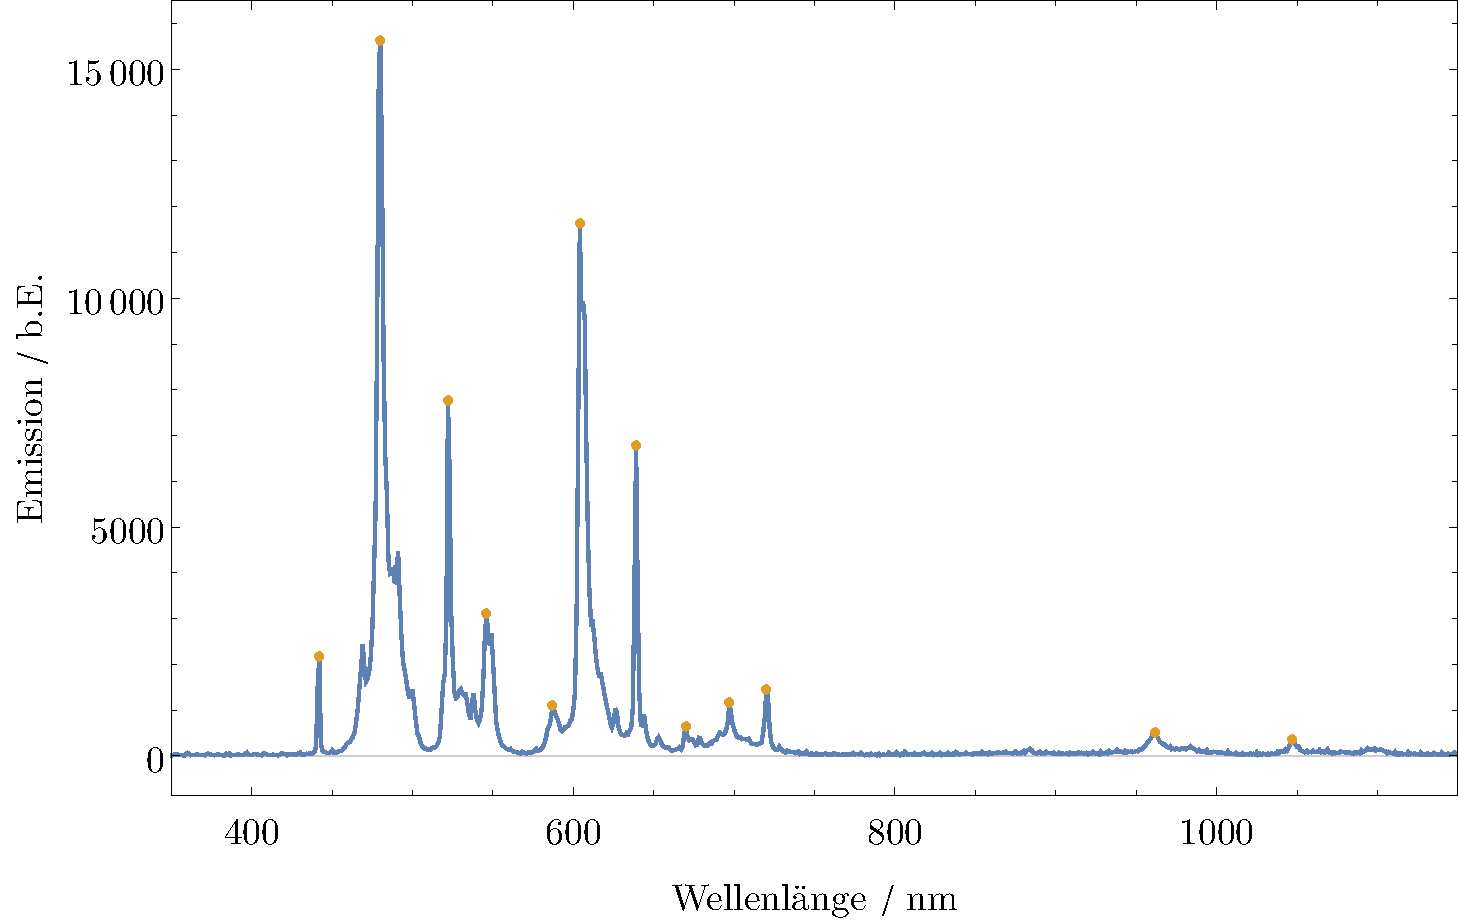
\includegraphics[width=\textwidth]{EmSpec.pdf}
  \caption{Emissionsspektrum des Pr:YLF-Kristalls und Position der Maxima.}
  \label{img:EmSpec}
\end{center}
\end{figure}

\begin{table}[htb]
\caption{Positionen und relative Intensitäten der Emissionsmaxima im Spektrum des
Pr:YLF-Kristalls.}
\begin{center}
\begin{tabular}{|c|c|}
\hline
Wellenlänge / nm & Emission / b.E. \\ \hline
442 & 2168.6 \\ \hline
480 & 15633.9 \\ \hline
522 & 7761.3 \\ \hline
546 & 3115.6 \\ \hline
587 & 1099.0 \\ \hline
604 & 11627.5 \\ \hline
639 & 6787.0 \\ \hline
670 & 635.9 \\ \hline
697 & 1162.8 \\ \hline
720 & 1457.7 \\ \hline
962 & 508.6 \\ \hline
1047 & 366.7 \\ \hline
\end{tabular}
\end{center}
\label{tab:EmSpec}
\end{table}


\FloatBarrier


\subsubsection{Messung der Lebensdauer des angeregten Zustands}

\paragraph{Aufbau und Durchführung}

\paragraph{Auswertung}



\subsubsection{Messung der absorbierten Leistung}

\paragraph{Aufbau und Durchführung}

\paragraph{Auswertung}
